\documentclass[]{scrreprt}
\usepackage{listings}
\usepackage{graphicx}
\lstset{numbers=left}
%opening
\title{Systemsicherheit - 3. Übung}
\author{Dennis Rotärmel, Niklas Entschladen, Tobias Ratajczyk, Gruppe Q}

\begin{document}

\maketitle
\pagebreak

\section*{Aufgabe 1: Size Directives}
\renewcommand{\labelenumi}{\alph{enumi})}
\begin{enumerate}
	\item optional
	\item erforderlich
	\item erforderlich
	\item optional
	\item fehlerhaft
\end{enumerate}

\section*{Aufgabe 2: Data-Only Attack}
\begin{figure}[h]
\centering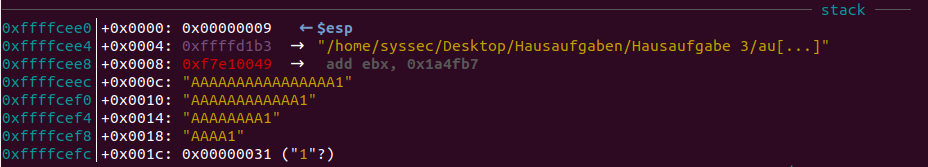
\includegraphics[width=1.1\textwidth]{images/1_bo_success.png}
\caption{\label{fig:bosuccess}Erfolgreicher Buffer Overlow}
\end{figure}
Wie in Abbildung \ref{fig:bosuccess} zu sehen ist, ist eine Data-Only Attack in dem bereitgestellten Programm möglich. Als Eingabe dienen hierbei 16 "{}A"{}Zeichen, welche das Array \verb|password_buffer| füllen. Die Größe des Buffers ist hierbei der Größe des Arrays zu entnehmen und beträgt 128 Bytes. Zusätzlich wird eine "{}1"{} an den übergebenen String angefügt, welche den Wahrheitswert der Variablen \verb|auth_flag| auf wahr setzt. \newline
Durch Tausch der Zeilen 8 und 9 ändert sich auch die Reihenfolge, in welcher die lokalen Variablen der Funktion auf den Stack gelegt werden.
Somit liegt (vorausgesetzt, dass hohe Adressen "oben" liegen) das übermittelte Passwort über der Variablen, welche eine erfolgreiche Authentifizierung kennzeichnet.
Eine Authentifizierung mithilfe eines Buffer Overflows wie zuvor ist somit nicht mehr möglich, da jene Variable nun nicht mehr überschrieben werden kann. 
\begin{figure}[h]
\centering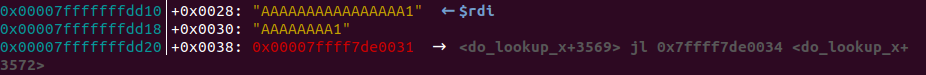
\includegraphics[width=1.1\textwidth]{images/2_bo_failure.png}
\caption{Hier funktioniert die zuvor verwendete Methodik nicht}
\end{figure}

\section*{Aufgabe 3: Shellcode}

\section*{Aufgabe 4: Stack-Based Buffer Overflow}

\section*{Aufgabe 5:  Smashing the Stack for Fun and Exam Prep}
	
\end{document}
